\documentclass[UTF8]{ctexart}
% \usepackage{xeCJK}
\usepackage{cancel}
\usepackage{graphicx}

\newcommand{\faq}[1]{{\heiti #1}}

\title{\textbf{北邮沙河生存手册R}}
\author{北邮软件工程根据地\ 群\thanks{主要贡献者(排名不分先后):甲、乙、丙、丁}}
\date{Rev.2.0(alpha), July 2022}

\begin{document}

\maketitle
\section*{声明}
\begin{center}
本内容以“CC BY-SA 4.0”许可证共享。要查看该许可证,可访问\\
https://creativecommons.org/licenses/by-sa/4.0/

受相关政策变化影响,部分内容可能有失准确,请以学校方面要求为准。
\end{center}
\tableofcontents
\newpage

\section{新生报道}

\subsection*{学号与班号}

首先欢迎2022级软件工程的同学们加入这个豪华孤儿院大家庭!
当你正式来到北邮的时候,便会得到两串十位数字:学号和班号。我们依次解读:
\begin{itemize}
    \kaishu
    \item 学号:2022(年份)21(全日制本科生)XXXX(四位学生编号)
    \item 班号:202121(同上)13(计算机学院\footnote{计算机学院(国家示范性软件学院)})16/17/18/19/20(软件工程的五个班\footnote{按照2021年的分班方法,这五个班以及一个双培班会成为四大班})
\end{itemize}

当你接触许许多多的新账号时,优先尝试账号为学号,密码为身份证后6/8位的组合,能解决80\%的问题。(注意,身份证号含有X的需要大写)

\subsection*{报道时间}

{\heiti 【待修改】开学时间节点(2021年)}
\begin{itemize}
\kaishu
    \item 8月27日 报道
    \item 8月29日 9:30-11:00 2021级本科生英语入学分级及免修资格考试
    \item 8月30日-9月12日 沙河校区校内军训
    \item 9月13日 正式第一天授课
\end{itemize}

报道当天会有志愿者在北京站、北京南站、北京西站给坐火车的同学们接站,到学校以后也会有志愿者(就是学长们啦)全程接驾,千万不要紧张哦~

\section{校区环境}

北邮现在使用中的校区一共两个,即海淀校区(西土城,本部)和昌平校区(沙河)。校本部位于海淀区西土城路10号,面积很小,住宿条件相对较差,但交通便利,对面就是北师大,周围没事众多。目前,大三大四的本科生及多数研究生在本部学习。沙河校区是新生入学的校区,位于昌平区沙河镇南丰路{\small{}与高教园南三街交口向北400米路东(我知道写这些你不会看的)}。规划面积很大(大概本部三倍)但是实际建成只有一半左右,住宿学习环境好,但比较偏僻,被两个地铁站夹在中间导致出行不便。沙河校区主要容纳大一大二学生。

按照学校最新的安排,计算机学院包括软工在内的学生都将只在沙河待一年,大二的时候就会搬到本部,所以今年沙河就只有22级的新生啦。

\begin{center}
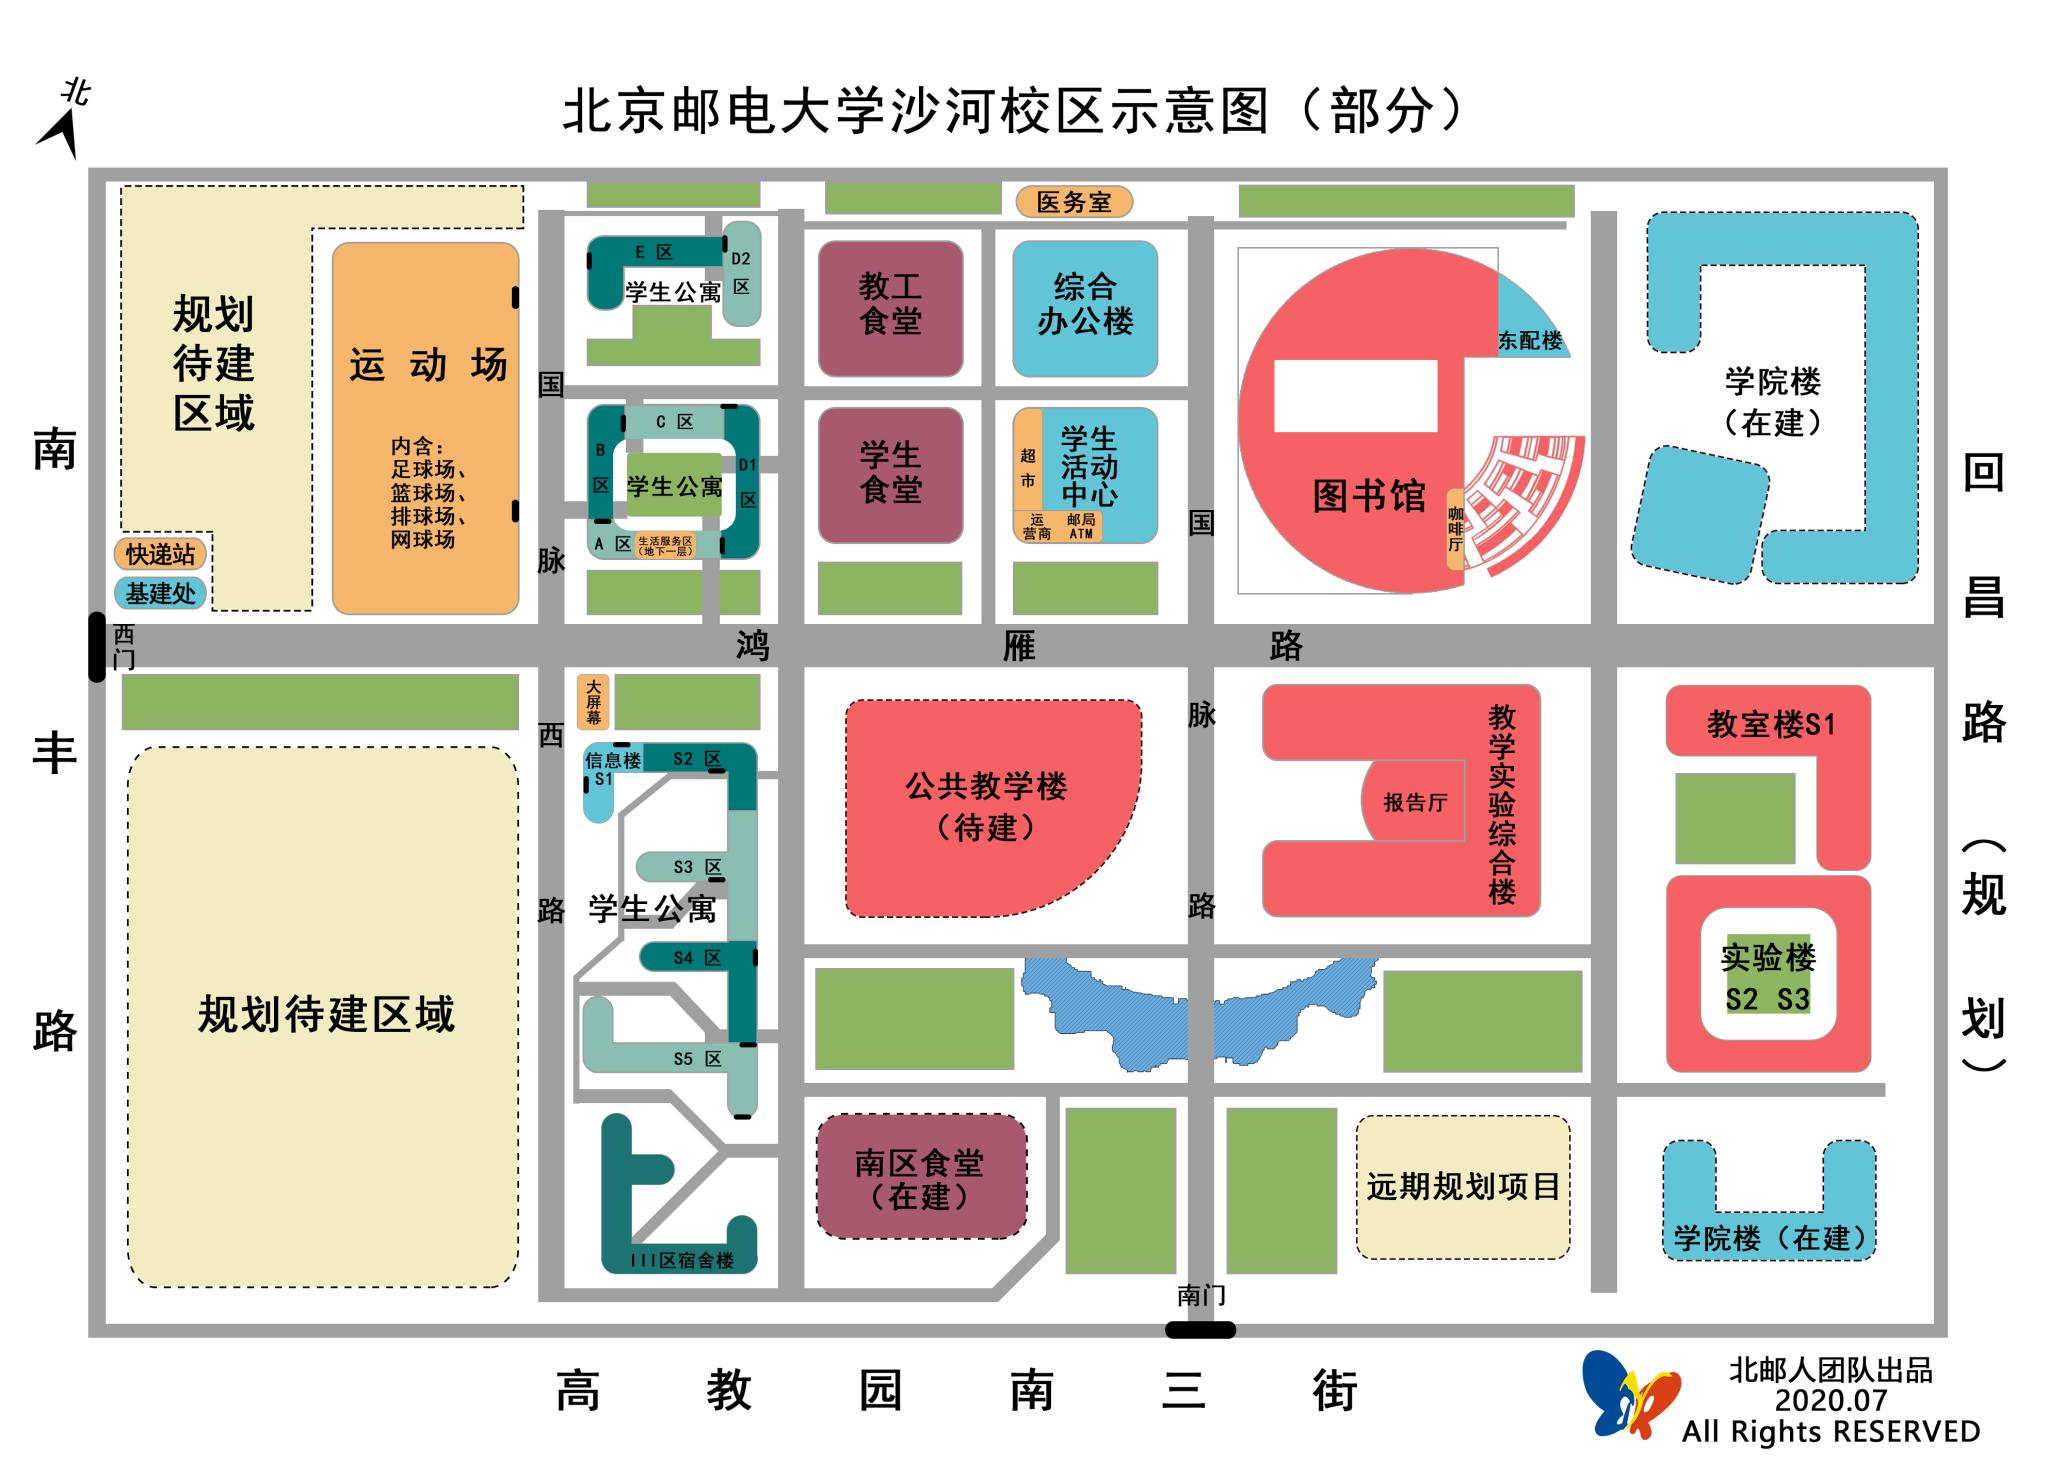
\includegraphics[width=0.80\textwidth]{images/shahe-map.png}
\end{center}

\faq{校园到底有多大?绕一圈要多久?}

很小,真的很小。本部绕一圈仅需10分钟,沙河大概也就20分钟(由于四周还没建设完成,所以(从物理上)根本无法绕圈(笑))。{\small (不过小也有小的好处,比如说可以7:55起床去上8:00的课)}

\faq{我什么时候会从沙河搬到本部?}

学校已经在招生章程中修改了各专业的办学地点。从2022级本科生开始,大部分学院(包括计算机学院在内)的大一会在沙河校区完成,大二至大四均会在校本部就读。

\faq{学校现在疫情管控严吗?能不能出去玩啊?}

根据学校目前的政策,出入校采取备案制(但疫情严重时会改为审批制,需要导员同意),不隔夜的情况下自动审批,大家白天出校门应该是没问题啦!关于疫情防控,现在学校内主要措施是进出建筑要戴口罩、测体温和扫二维码,部分食堂的桌子上有隔板,建议大家错位就餐哦(当然也不强制)。上课、体育锻炼和取快递外卖不受影响。

当然,入学后一定会有每日填报信息,大家不要忘哦。虽然也有自动打卡脚本,不过目前严抓,大家还是动动小手自己打卡吧~

\faq{有校车吗?免费吗?}

有,校车往返本部和沙河,但只在工作日安排。学期开始后可以在学校公众号上查询具体班次。由于校车要优先服务老师和本部学生,所以有可能会没有位子。有部分时段的校车需要提前在公众号上预约。

车费5元,比地铁便宜。正常情况下需用时35-55分钟,相较于地铁会更快一点。

\faq{寒暑假我可以住在学校吗?}

目前由于学校规划调整,两个校区寒暑假都不再封校,但受疫情影响可能难以通过假期留校审批。另需支付住宿费。

\section{住宿条件}

\subsection*{沙河宿舍简介}

根据宿舍楼的位置,沙河校区的宿舍分为雁北园和雁南园。相对而言,雁北园的条件会差一些,比如阳台空间较小、公共浴室较为破旧和储物空间较少。但其实也只是差一点~

\emph{雁北园}位于鸿雁路北侧,A/B/C/D1是四栋矩形相连的宿舍楼(一楼入口独立,二楼以上的部分相连),D2/E是另两栋独立于A/B/C/D1宿舍楼且相对较小的宿舍楼,内部也是相连的。目前2020级软件工程的学长们就住在这里(等你们入学就要搬去本部了),离食堂操场生活区较近。雁北园各区域的代号为A/B/C/D1/D2/E。

\emph{雁南园}位于鸿雁路南侧,S2 S3 S4 S5是四栋平行的宿舍楼,六层,是2021级学生的主要宿舍楼,离教学楼和学校景观湖(线程池?)较近,南区食堂也修好了,即将投入使用。S6是一栋单独的宿舍楼,由于2020年才投入使用,所以条件是全校最好的。雁南园各区域的代号为S2/S3/S4/S5/S6(S1是信息中心楼)。
注:
学校有三栋教学楼的名字也是S1、S2和S3,不要和宿舍楼弄混哦~
S2 S3 S4 为男生宿舍,互通
S5 S6为女生宿舍(实际有三个不相通的部分)
按照学校的安排,之后所有的女生应该会统一入住S5和S6,其余宿舍均为男生宿舍。

\subsection*{宿舍环境}

无论是雁北园还是雁南园,宿舍的基本配置都是:四人间,上床下桌,有独立卫生间。卫生间内只有一个坑位和洗脸面盆,不能洗澡(但有地漏)。有的宿舍楼的独立卫生间会分成两个部分,分别是坑位和洗脸池。厕所里没有垃圾桶,需要自己购买。房间内有空调和暖气片,有阳台。

\begin{center}
\begin{minipage}{0.45\textwidth}
    \centerline{\fangsong\small 雁北和除S6以外的雁南宿舍}
    \centerline{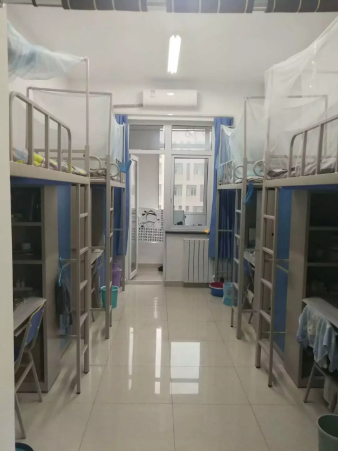
\includegraphics[width=1\textwidth]{images/dorm.png}}
\end{minipage}
\qquad
\begin{minipage}{0.45\textwidth}
    \centerline{\fangsong\small 雁南S6宿舍}
    \centerline{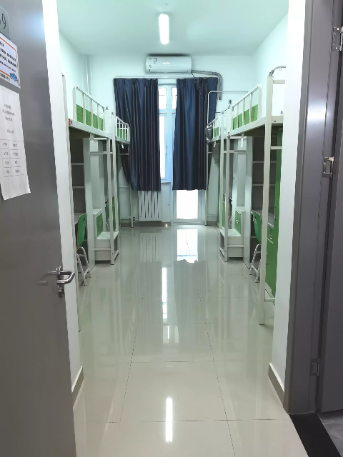
\includegraphics[width=1\textwidth]{images/dorm-s6.png}}
\end{minipage}
\end{center}

\faq{我需要带什么生活用品吗?}

其实你可以什么也不带,报道当天都可以去学校超市购买。当然你自己带好常用的洗漱用品、床单被套啥的也可以。(建议非必须物品提前物流、网购或现场买,不建议千里迢迢携带)

\faq{宿舍楼还有其他配置吗?}

每层楼有一个公共卫生间和澡堂,(如果不想经常清理房间里的厕所,建议多去公共卫生间),一楼有宿管的值班室,可以使用微波炉。每栋楼有一个电梯,一楼有若干自动售货机(买饮料零食泡面啥的),支持移动支付。部分楼层会有空出的房间作为自习室。

\faq{宿舍楼有门禁吗?}

有,同一栋楼仅允许该楼学生刷卡进入,实际没有,但有宵禁。宿舍楼开放时间是早上6点到晚上11:00,如果要十一点以后回宿舍,就要提前联系辅导员进楼。带外来人员进楼要在宿管处登记。

\faq{澡堂是怎么样的?}

纯淋浴房。采用刷卡计费的方式,大概每分钟0.1元。澡堂中午12:00到晚上23:00开放(其实管的不严的情况下一般不锁门,但最好还是提前去洗),但一般下午四五点以后才有热水。实测全天有热水,多放一会儿即可。

\faq{我会和我的同班同学住一个寝室吗?}

一般会,但也可能和同专业的其他班同学住一起。极端情况下你会与其他专业的同学一个寝室。分寝室结果在报道前可以在信息门户网上查到。

\faq{水电费怎么算?}

水费目前没有收。电费每人每学期赠送40度电。(所以宿舍四个人一共赠送160度)电费价格:12元可购买25度电。(只有空调最花钱,要不然花不了多少电)

\faq{宿舍装饰有什么限制吗,可以拉床帘吗?}

规定上不允许安装床帘,实际执行上不严。有部分宿管会限制蚊帐、床帘和地垫,可以尝试和他们理论,无果的话就不要装啦,具体购买之前可以先询问宿管和辅导员。不可以使用大功率电器(具体到时看宿舍须知)

\faq{上床下桌的尺寸是多大?}

\begin{center}
    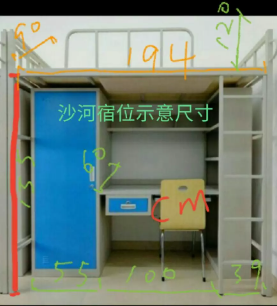
\includegraphics[width=0.6\textwidth]{images/bed-size.png}
\end{center}

又到了搬出老图的时候——不同宿舍的柜子尺寸可能不同,上床离天花板大概一米多一点,桌子上可以放得下27"显示屏。

\faq{辅导员会检查宿舍吗?}

辅导员开学后会有宿舍评比,主要看装饰和整洁度,可能会影响德育分(关于德育分的问题见下),具体看学院政策。辅导员查寝的频率取决于你的导员有多懒,以及学院有没有发动什么相关运动。
每周会有宿管卫生检查(实际上没来过几次),按百分制进行计分,基准分为100不符合规定的倒扣对应分数。

\section{学业相关}
\section{生活相关}
\section{军训相关}
\section{内网资源}
\section{学生组织}
\section{其他事项}

\end{document}
